\documentclass[]{vgtuef}
\usepackage[utf8x]{inputenc}
\usepackage[L7x]{fontenc}
\usepackage[lithuanian]{babel}


\author{Tomas Fedosejev, Marius Buinevičius\\Vilniaus Gedimino technikos
  universitetas\\Elektronikos fakultetas\\Elektroninių sistemų
  katedra\\\texttt{tomas@fedosejev.lt}}
\title{Bakalauro baigiamasis darbas\\Virtualios garso realybės sistema}


\begin{document}

\setcounter{page}{7}
%\setcounter{totalnumber}{4}
\onehalfspacing

\tableofcontents


\section*{Žymenys ir santrumpos}
\addcontentsline{toc}{section}{Žymenys ir santrumpos}

\begin{itemize}
\item MARG -- Magnetinis laukas, kampinis pagreitis ir laisvojo kritimo pagreičio vektorius (angl. \textit{Magnetic, Angular Rate, and Gravity})
\item HRTF -- su galva susijusios perdavimo funkcijos (angl. \textit{Head Related Transfer Function}).
\item ATF -- anatominė perdavimo funkcija (angl. \textit{Anatomical Transfer Function}).
\item FFTF -- (angl. \textit{Field-Free Transfer Function}).
\item RIR -- kambario impulsinis atsakas (angl. \textit{Room Impulse Response}).
\item HRIR -- (angl. \textit{Head Related Impulse Response}).
\item ITD -- tarpausinis laiko skirtumas (angl. \textit{Interaural Time Difference}).
\item ILD -- tarpausinis garso lygių skirtumas (angl. \textit{Initial Level Difference}).
\item USB -- universalioji nuoseklioji jungtis (angl. \textit{Universal Serial Bus}).
\item COM -- RS232 nuoseklusis prievadas.

\end{itemize}

\section{Įvadas. Užduoties analizė}

Darbo tema yra „virtualios garso realybės sistema“. Šiuo metu virtuali ir papildytos realybės programinė įranga yra toli pažengusi, tačiau garso generacijai taip ir toliau naudojamas stereo garsas, kuriuo nėra įmanoma tiksliai atkurti aplinkos garsų.

Šiuo darbu siekiama ištirti galimybes sukurti realiuoju laiku veikiančia sistemą gebančią generuoti binauralinį garsą priklausomai nuo vartotojo galvos orientacijos ir virtualios aplinkos akustinių parametrų. Sistema yra suskirstyta į tris pagrindines dalis: galvos sekimo įrenginys -- kuris seka vartotojo galvos orientaciją; programa asmeniniame kompiuteryje -- kuri siunčia virtualios aplinkos duomenis ir garso šaltinio skleidžiamą garsą; garso apdorojimo įrenginys -- kuris apjungia informaciją gautą iš galvos sekimo įrenginio bei asmeninio kompiuterio ir sugeneruoja binauralinį garsą. Tokia architektūra buvo pasirinka dėl modulinės struktūros, be to perkėlus garso generavimą į atskirą įrenginį, atlaisvinamas asmeninio kompiuterio centrinis procesorius, ko pasėkoje virtualiai aplinkai sukurti lieka daugiau asmeninio kompiuterio resursų.

Pradiniai bandymai bus atlikti \textit{Matlab} terpėje, kas leis įsitikinti sistemos įgyvendinimo galimybėmis, bei duos progą patobulinti naudojamus procesus.

Virtualios garso realybės tema buvo pasirinkta dėl savo perspektyvumo, nors binauralinis garsas pradėtas tirti pakankamai senai, realiai veikiančių įrenginių nėra sukurta. Tema yra aktuali žaidimų ir medicinos pramonei.

Didžiausia sistemos problema slypi HRTF (angl. \textit{Head Related Transfer Functions}) panaudojime, kadangi HRTF deriniai turi būti pritaikyti individualiai kiekvienam klausytojui. Tačiau panaudojus papildomus procesus garso generavimo eigoje, pamėginta sumažinti HRTF neigiamą įtaką.

Darbo eigoje bus sukurta pilnai veikianti sistema gebanti kuo tiksliau atkurti virtualią akustinę aplinką, programinė įranga bus parašyta garso apdorojimo, galvos orientacijos įrenginiams, bei asmeniniam kompiuteriui. Taip pat bus suprojektuoti abu naudojami įrenginiai.

Baigiamojo bakalaurinio darbo sistemos asmeninio kompiuterio programinei įrangai reikalingi mažiausiai 20MB diskinio kaupiklio dalies talpos. Toks atminties kiekis reikalingas norint vartotojo sąsają padaryti patrauklesnę vartotojui, t.y. grafinės iliustracijos, garsai ir kt. Asmeniniame kompiuteryje programinė įranga dirba \textit{Windows 7} operacinėje sistemoje, nes senesnių operacinių sistemų versijų (\textit{XP}, \textit{Vista}) Microsoft korporacijos palaikymas bus nutraukiamas artimiausiu metu.

Garso apdorojimo įrenginyje bus naudojama ne mažesnė nei 1.1 \textit{USB} lizdo versija, nes sistema suprojektuota darbui su šia ar aukštesnėmis versijomis. Duomenų perdavimą taipogi būtų galima realizuoti ir kitomis sąsajomis, tokiomis kaip \textit{COM}, bet tokiu atveju greitis būtų nepakankamas ir sistema įgautų netoleruotiną vėlinimą. Be to, binauralinio garso generavimo sistema yra šiuolaikinė ir labiau taikintina nešiojamiems kompiuteriams, kuriuose nebediegiami \textit{RS232} prievadai. Išlieka galimybė naudoti \textit{RS232} prievadą, bet tokiu atveju tektų papildomai turėti iš \textit{USB} į \textit{COM} keitiklio kabelį, kuris taip pat naudoja \textit{USB} jungtį. Todėl geriausias pasirinkimas spartos atžvilgiu rinktis virtualų \textit{COM}  prievadą per \textit{USB} jungtį.

Siekiant išlaikyti kuriamos sistemos kuo ilgesnį autonominio veikimo laiką sistema toleruoja maksimalų 0,5 A srovės suvartojimą (tiek galvos orientacijos nustatymo įrenginys, tiek garso apdorojimo įrenginys), be to 0,5 A tai didžiausia srovė kurią pagal specifikaciją gali atiduoti \textit{USB 1.1} ir \textit{USB 2.0} prievadai.

Norint išlaikyti sistemos mobilumą, kurio didžioji dalis priklauso nuo galvos sekimo įrenginio dydžio, buvo pasirinkti pakankamai nedideli pastarojo įrenginio maksimalūs matmenys: 50 $\times$ 100 $\times$ 100 mm.

Sistemos veikimas bus vertinamas sugeneruoto binauralinio garso tikslumu (palyginus su įrašytu binauraliniu garsu), bei autonominio veikimo trukme.


\section{Analogiškų sistemų apžvalga}

Šiame skyriuje bus apžvelgtos analogiškos sistemos: buvę prototipai ir šiuo metu esami rinkoje produktai. Apibendrintai bus aptarti nagrinėjamų sistemų teigiamos ir neigiamos savybės. 


Galvos sekimo įrenginio kūrimas nėra naujiena. Tokie įrenginiai naudojami norint nustatyti lėktuvų  trimatę poziciją. Pati \textit{sensor fusion} technologija taip pat jau gana ilgai naudojama aviacijos srityje, norint kur kas tiksliau nustatyti poziciją.

Kalbant apie binauralinio garso generavimą realiu laiku, paieškos rezultatai stipriai sumažėja. Tokio tipo projektų pasaulyje yra tik du. Projekto tikslas – binauralinio garso generavimas realiu laiku. Vienas iš projektų naudojo \textit{„Texas instruments“} pagamintą plokštę -- C6713 DSK kuri pavaizduota \ref{fig:C6713_dsk_board} pav.

\begin{figure}[!ht]
  \centering
  \includegraphics[width=390px]{img/c6713.jpg}
  \caption{C6713 DSK spausdintinė plokštė.}
  \label{fig:C6713_dsk_board}
\end{figure}

Šios plokštės mikrovaldiklis dirba 225 MHz dažniu ir pasiekia 1800 milijonų instrukcijų per sekundę spartą. Taip pat ši plokštė gali atkurti aukštos kokybės 24 bitų skaitmeninį stereo garsą, turi 512 kB \textit{Flash} bei 16 MB \textit{SDRAM} atminties. \textit{JTAG}\footnote{JTAG -- Programavimo ir testavimo jungtis.} prieinamas per \textit{USB} jungtį.

Kaip teigia gaminio kūrėjai, jie generuoja binauralinį garsą naudojant specialų stereo filtrą suprogramuotą minėtoje plokštėje. Programinė įranga naudoja HRTF sugeneruotas \textit{„Floridos tarptautinio universiteto“} asmenų (nepaminėta kieno). Dviejų kanalų išėjimui panaudotos 12 \textit{HRTF} funkcijų, kurios taip pat nebuvo sugeneruotos projekto autorių. 

Kūrėjų teigimu, rezultatai jų stipriai nestebina – geriausias efektas jaučiamas tik garsui esant už galvos, nes panaudotos \textit{HRTF} funkcijos nėra pritaikytos jų ausims. Šio įrenginio testavimo akimirką demonstruoja \ref{fig:C6713_dsk_board_checkout} pav.

\begin{figure}[!ht]
  \centering
  \includegraphics[width=390px]{img/c6713_patikra.jpg}
  \caption{C6713 DSK plokštės patikra.}
  \label{fig:C6713_dsk_board_checkout}
\end{figure}


Kompiuterinis binauralinio garso generavimas yra įmanomas, bet reikalauja didelių kompiuterio resursų, taip atimdamas galią iš centrinio procesoriaus, todėl kuriamos išorinės garso plokštės, kurios nepriklausomai nuo kompiuterio procesoriaus gali generuoti binauralinį garsą naudojant \textit{HRTF} funkcijas.

Pirmoji garso rinkoje pasirodęs produktas, galėjęs pasiūlyti trimatį pozicinį garso generavimą, buvo 1998 išleista \textit{„Aureal Vortex via the A3D API“} garso plokštė. Deja nėra  galimybės jos išbandyti, bet pagal vartotojų atsiliepimus ši plokštė sugebėdavo gana gerai suformuoti trimačio garso pojūtį. Kadangi įmonė \textit{„Aureal“} pasitraukė iš rinkos, tai jos poziciją perėmė \textit{„Creative Inc.“} firma. Gerą garso kokybę bei neblogą trimačio garso efektą gali pasiūlyti tik labai brangios pastarosios įmonės garso plokštės – \textit{„X-Fi“}. 

Šiuo metu binauralinio garso generavimas realiu laiku priklausomas nuo vartotojo galvos pozicijos neturi jokių analogų. Kaip ir buvo minėta, atskirai abi dalys yra daugiau ar mažiau naudojamos pasaulinėje rinkoje, bet būtent šių dviejų sričių sujungimas yra visiškai unikalus, todėl analogiškų sistemų apžvalga čia yra neįmanoma.

Kaip buvo minėta apžvalgoje sistema pasiūlytame pavidale yra unikali ir perspektyvi. Šiuo metu rinkoje nėra įrenginių gebančių sugeneruoti bunauralinį garsą priklausomai nuo klausytojo galvos orientacijos. Rinkoje esantys analogai suteikia programuotojams galimybę įgyvendinti šį efektą naudojantis papildomais programiniais įrankiais, tačiau įrenginių gebančių tai padaryti savaime, be papildomo programuotojų įsikišimo -- nėra.

\section{Naudojamų metodų apžvalga}
\label{sect:naudojami_metodai}

Šiame skyriuje bus apžvelgti metodai kuriais remiantis buvo sukurti matematiniai modeliai ir realios sistemos prototipas.

\subsection{HRTF funkcijos}

\textit{HRTF} (angl. \textit{Head Related Transfer Function}) dar vadinamos \textit{ATF} (angl. \textit{Anatomical Time Difference}) tai funkcijos nusakančios atsaką kurį kuris charakterizuoja, kaip žmogaus ausis priima garsą sklindantį iš tam tikro taško erdvėje. Panaudojus \textit{HRTF} porą, skirta kiekvienai ausiai, įmanoma sintezuoti binauralinį garsą taip sukuriant erdvės pojūtį.  
Žmogaus smegenys apskaičiuoja garso šaltinio poziciją erdvėje naudojantis: 1) garso užuominomis atkeliavusiomis į kiekvieną ausį (angl. \textit{monoaural cues}), 2) abiejų ausų garso užuominų palyginimu (angl. \textit{difference cues} arba \textit{binaural cues}). Pagrindinės garso užuominos yra:
\begin{enumerate}
\item Tarpausinis laiko skirtumas (angl. \textit{Interaural Time Difference})
\item Tarpausinis garso lygių skirtumas (angl. \textit{Interaural Level Difference})
\item Spektriniai skirtumai (angl. \textit{Spectral cues} arba \textit{Pinae effect})
\item Galvos šešėlis (angl. \textit{Head Shadow})
\item Pečių aidas (angl. \textit{Shoulder Echo})
\item Ankstyvieji atspindžiai (angl. \textit{Early Reflections})
\item Atgarsiai (angl. \textit{Reverberation})
\end{enumerate}

\textit{HRTF} aprašo tik dalį iš aukščiau pateiktų užuominų: TLS ir TGLS.


\subsection{Galvos šešėlis ir pečių aidas}

Galvos šešėlis arba dar kitaip vadinamas akustiniu šešėliu, tai sumažėjusios garso amplitudės regionas atsirandantis, nes galva sugeria arba sumažina amplitudę dalies ją pasiekusių garso bangų. Pasiekusi galvą garso banga gali keliauti aplink arba per galvą, kad pasiektų ausį esančią priešingoje pusėje. Tokiu būdu yra sukuriamas pakankamai geras pirminės lokalizacijos filtras. Ausį esančią šešėlyje garsas pasiekia maždaug 0,7 ms vėliau, ko pasėkoje žmogaus smegenys sugeba nustatyti apytikslią garso sklidimo kryptį. 

Pečių aidas -- tai aidas atsirandantis garso bangom atsispindėjus nuo klausytojo pečių. Toks aidas tiesiogiai turi mažai lokalizacijos informacijos tačiau sudėjus kartu su galvos šešėliu filtras dar labiau patikslėja.


\subsection{Tarpausinis laiko skirtumas}

TLS nusako laiko skirtumą tarp garso bangų pakliuvusių į dešiniąją ir kairiąją ausis, \ref{fig:ITD_1} paveikslas vizualiai parodo šio efekto veikimą. TLS – tai pirminė garso lokalizacijos užuomina padedanti nusakyti garso šaltinio padėtį erdvėje. Kadangi ausys yra atskirtos viena nuo kitos, garso banga nukeliauja skirtingą kelia prieš pasiekiant kiekvieną iš ausų.

\begin{figure}[!ht]
  \centering
  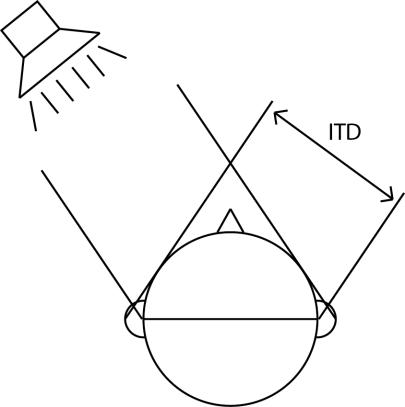
\includegraphics[width=150px]{img/ITD.jpg}
  \caption{TLS (angl. \textit{ITD}) efektas}
  \label{fig:ITD_1}
\end{figure}

Tačiau išimtį sudaro garsas esantis tiesiai prieš arba už klausytojo. TLS taip pat įtakoja garso bangos fazės  pakitimą. Jeigu fazių skirtumas didesnis nei 180 laipsnių, nustatyti kaip fazė yra pasislinkus tampa sunku. Žemuose dažniuose fazės skirtumas nusako pakankamai didelį laiko skirtumą ir yra naudingas orientacijos nustatymui. Aukšto dažnio signalams 180 laipsnių fazės poslinkis  nusakys mažesnį laiko skirtumą. Tai reiškia kad ši savybė tampa mažiau naudinga garso bangoms kurių dažnis priklausomai nuo kampo viršija 700-1500 Hz.

\subsection{Tarpausinis garso lygių skirtumas}
TGLS nusako garso stiprumo skirtumą tarp dviejų taškų (ausų). Šis reiškinys pasireiškia kai garso banga iš dalies yra blokuota galvos. Taip pat kaip ir TLS, TGLS negali tiksliai nusakyti skirtumo tarp garso esančio tiesiai prieš arba už klausytojo. TGLS efektas taipogi kaip ir TLS turi dažninę priklausomybę. Žemuose dažniuose dėl difrakcijos tik maža garso bangos dalis yra blokuota galvos, ko pasėkoje garso intensyvumo skirtumas pasidaro labai mažas.

Tačiau aukštų dažnių ruože difrakcija pasireiškia žymiai mažiau kas įtakoja žymiai didesni garso lygių skirtumą (\ref{fig:ILD_1} paveikslas). Kai kuriais atvejais garso lygių skirtumas gali sudaryti iki 20 dB. Todėl TGLS yra dažniausiai naudojamas aukšto dažnio garso bangoms, o TLS žemo dažnio bangų krypčiai nustatyti. 

\begin{figure}[!ht]
  \centering
  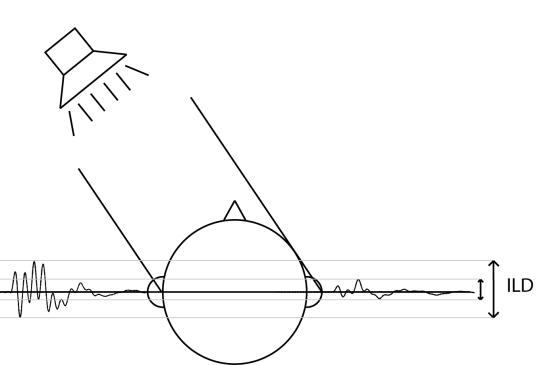
\includegraphics[width=150px]{img/ILD.jpg}
  \caption{TGLS (angl. \textit{ITD}) efektas}
  \label{fig:ILD_1}
\end{figure}

Taipogi labai svarbi yra spektrinė dedamoji (angl. \textit{pinnae effect}). Dėl kompleksinės ir asimetrinės ausies kriauklės formos garsas atsispindėjęs nuo ausies kriauklės spektriškai pasikeičia.  Kartu su pečių atspindžio efektu tai formuoja filtrą turintį krypties priklausomybę ir todėl ne taip kaip TLS ir TGLS yra įmanoma atskirti garsus sklindančius iš priekio ir iš galo. Dėl spektrinių pokyčių ši dedamoji geriausiai tinka atskirti plačiajuostį garsą -- viršijantį 6 kHz dažnį.


\subsection{HRTF metodo panaudojimas}

Norint panaudoti šį metodą reikia turėti \textit{HRTF} rinkinį visiems vertikalių ir horizontalių kampų deriniams. Šiame darbe naudojami Masačiuseco technologijų instituto (angl. \textit{Massachusetts Institute of Technology}) 1994 metais atlikto projekto \textit{„KEMAR“} metu gauti universalūs \textit{HRTF} deriniai.

Turint baigtinio ilgio skaitmeninį garso signalą atliekama diskrečioji sąsuka (angl. \textit{convolution}) pagal \ref{equ:conv_1} formulę:

\begin{equation}
(f * g)[n] = \sum_{m=0}^{\infty} f[m]*g[n-m]=\sum_{m=0}^{\infty} f[n-m]*g[n]
  \label{equ:conv_1}
\end{equation}

čia $f$ – vieno kanalo baigtinio ilgio daugianaris (angl. \textit{polynomial}), $g$ – atitinkamo kanalo \textit{HRTF} funkcija (išreikšta daugianariu), $n$ – daugianario narių skaičius.

Šioje formulėje atliekama dviejų daugianarių daugyba, rezultate gauto daugianario koeficientai atitinka originalaus daugianario ($f$) koeficientų seką po sąsukos, visi likę nežinomi koeficientai yra prilyginami nuliui kad nekiltų neapibrėžtumas. Šis veiksmas dar žinomas kaip dviejų daugianarių koeficientų Kauči daugyba (angl. \textit{Cauchy product}).

Veiksmas atliekamas atskirai dešiniajam ir kairiajam kanalams naudojant tą patį garso signalą su atitinkamai dešiniajai arba kairiajai ausiai skirta \textit{HRTF} funkcija.

\subsection{Duplekso teorija}

Duplekso teorija, pateikta Lordo Reilėjaus (Lord Rayleigh), pateikia paaiškinimus apie žmogaus galimybę lokalizuoti garsus pagal laiko skirtumą TLS tarp garsų, patenkančių į kiekvieną ausį ir taip pat skirtingo garso lygio TGLS patekimą į ausis. Bet iki šiol išlieka klausimas, ar šie skirtumai yra pastebimi.

Duplekso teorija teigia, kad TLS naudojamas žemo dažnio garso šaltinio lokalizacijai, o TGLS – aukšto dažnio. Kadangi natūralus garsas sudarytas ne tik iš žemo dažnio komponenčių, bet ir aukšto dažnio, tai klausos sistema turės panaudoti abi metodikas (tiek TLS tiek TGLS), norint tiksliai nustatyti garso šaltinio vietą. Šios dupleksinės sistemos rezultatas – ji gali taip pat generuoti taip vadinamus „garso lokalizacijos užuominų mainų“  arba „laiko intensyvumo mainų“ dirgiklius ausinėse, kur TLS, nukreiptas į kairiąją ausinių pusę, perstumtas per TGLS, kuris savo ruoštu nukreiptas į dešiniąją ausinių dalį, todėl garsas suvokiamas lyg sklistų iš vidurio. Kaip ir visos teorijos, duplekso teorija taip pat susiduria su problemomis. Pastaroji negali iki galo paaiškinti kryptingo girdėjimo, o taip pat išlieka priekinio-galinio garso šaltinio padėties girdimumo problema. Taip pat ši teorija apima tik horizontaliąją garso šaltinio lokalizaciją aplink galvą. Dar vienas teorijos netikslumas – neatsižvelgimas į ausies kaušelio formą lokalizacijos paaiškinime.

1938 metais Vudvortas atliko eksperimentą, kuriame iš pilnavidurio rutulio buvo sumodeliuota žmogaus galva. Su šiuo modeliu buvo matuojami TLS kaip kampo su vertikalia plokštuma funkcija skirtingiems dažniams. Šiame galvos modelyje tarpas tarp dviejų ausų buvo apie 22 -- 23 cm. Pirminiai šio eksperimento rezultatai parodė, kad didžiausias laiko tarpas, per kurį garsas patenka iš vienos ausies į kitą, buvo apie 660 μs, kai garso šaltinis buvo padėtas lygiai 90$^\circ$ kampu vertikalios plokštumos atžvilgiu. Šis laiko tarpas susidaro, kai garso bangos dažnis siekia 1500 Hz. Rezultatai parodė, jog grojant garsui, kurio dažnis mažesnis nei 1500 Hz bangos ilgis yra didesnis negu minėtojo didžiausio laiko tarpo. Taigi rezultatai parodo, jog tarp garso bangų, patenkančių į ausis, atsiranda fazių skirtumas ir tai sukuria akustinės lokalizacijos užuominas. Garso dažniui artėjant prie 1500 Hz, garso bangos ilgis yra panašus į natūralų garso vėlavimą. Dėl galvos dydžio ir tarpo tarp ausų yra sumažėjęs fazių skirtumas, taigi iš karto atsiranda lokalizacijos paklaida. Garso dažniui esant didesniam nei 1500 Hz, garso bangos ilgis tampa mažesnis nei atstumas tarp ausų, tuomet atsiranda „galvos šešėlis“   ir GLS suteikia garso lokalizacijos užuominų.

Feddersen et al. atliko eksperimentus (1957 metais), kuriais jis matavo, kaip kinta LS, keičiant garsiakalbio kampą aplink galvą su vertikaliąja plokštuma, esant skirtingiems dažniams. Bet jo eksperimentai skyrėsi nuo „Woodworth“ tuo, kad Feddersen atliko tyrimus su realiais žmonėmis, o ne su galvos modeliais. Šio eksperimento rezultatai sutapo su Vudvorto gautais rezultatais. Tyrimo rezultatai taip pat parodė, kad nėra jokio TLS skirtumo tarp dviejų garso šaltinio pozicijų – kai garso šaltinis yra priešais galvą (0$^\circ$) ir už galvos (180$^\circ$). Tokių rezultatų paaiškinimas – garso šaltinio atstumas iki ausų yra vienodas abiem atvejais. Laiko skirtumas keičiasi tik garso šaltiniui keliaujant aplink galvą. Šiuo ekperimentu įrodyta, kad didžiausias laiko skirtumas yra 660 μs ir jis gaunamas, garso šaltinį padėjus šalia ausies. \ref{fig:ITD_1} paveiksle pavaizduotas galvos modelis ir garso šaltinio skleidžiamų garso bandų kryptis ir susidarantis kampas.

\ref{fig:ITD_1} pav. matoma, jog kelias nuo garso šalinio iki kiekvienos ausies yra skirtingas. Garso kelias iki kairės ausies yra didesnis, nei kelias iki dešinės ausies. Šis garso kelių skirtumas perkeltas į lauko ašį, nusako tarpausinį laiko skirtumą TLS.
TLS yra dominuojanti garso šaltinio lokalizacijos užuomina dažniams iki 1.5 kHz (imtinai). Visiems kitiems dažniams, didesniems nei 1.5 kHz dominuojanti užuomina yra tarpausinis garso lygio skirtumas TGLS. Tarpausinis garsio lygio skirtumas atsiranda dėl taip vadinamojo „galvos šešėlio“. Jis atsiranda tik prie aukštesnių dažnių, kuomet garso bangos nebesukelia difrakcijos aplink galvą, taip sukurdamos galvos šešėlį, kuris panašus į šešėlį, susidarantį krentant šviesos bangoms link galvos.

Norint įrodyti Lordo Reilėjaus teoriją, buvo atliktas eksperimentas, kuriame garso šaltinį ir manekeno galvą skyrė 1,75 m. Eksperimentas atliktas beaidėje aplinkoje. Jį atliko Levisas Skotas Diamondas (Lewis Scott Diamond).  Naudojant skirtingo dažnio – 125 kHz, 250 kHz, 500 kHz ir 1000 kHz programa Csound sugeneruotus garsus, kai garso signalo šaltinis buvo padėtas skirtingais kampais – 0$\circ$, 10$\circ$, 30$\circ$, 50$\circ$, 70$\circ$, 90$\circ$, pavyko įrodyti šią teoriją. \ref{fig:1000kHz_TGLS} paveiksle pavaizduota 100 kHz dažnio grynojo tono oscilograma.

\begin{figure}[!ht]
  \centering
  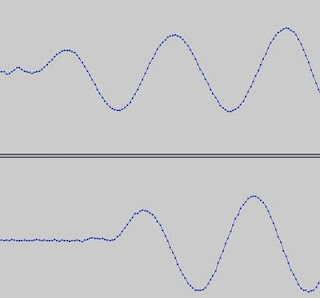
\includegraphics[width=250px]{img/100kHz_grynas.png}
  \caption{100 kHz grynojo tono gauto manekeno galvoje oscilograma (viršuje – kairioji ausis, apačioje – dešinioji}
  \label{fig:100kHz_grynas}
\end{figure}

\ref{fig:100kHz_grynas} pav. matomi grafikai atvaizduoja manekeno galvoje esančių mikrofonų parodymus, esant garso šaltinio skleidžiamam garsui, kurio dažnis siekė 1000 kHz ir atstumas iki jo – apie 1,75 m. Viršutinėje paveikslo dalyje – kairiosios ausies mikrofono oscilograma, apatinėje dalyje – dešiniosios. Iš paveikslo matome, jog tarp abiejų mikrofonų oscilogramose susidaro fazių skirtumas, taip pat apatinėje paveikslėlio dalyje matomas atsiradęs laiko vėlavimas lyginant su kairiosios ausies mikrofono grafiku. Signalo tarpausinis laiko skirtumas siekė 0,735 ms, ir tai yra didžiausias pasiekiamas laiko skirtumas, nes manekeno galvos priekinė dalis buvo statmena garso signalo šaltiniui. \ref{fig:TLS_degree} pav. pavaizduoti tarpausinio laiko skirtumo priklausomybių nuo skirtingo dažnio garso bangų grafikai.

\begin{figure}[!ht]
  \centering
  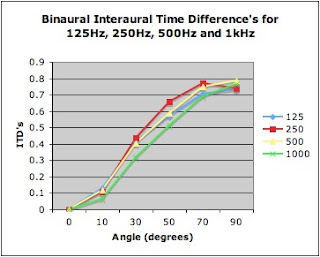
\includegraphics[width=300px]{img/TLS_degree.png}
  \caption{Tarpausinio laiko skirtumo priklausomybė nuo garso kritimo kampo.}
  \label{fig:TLS_degree}
\end{figure}

0,735 ms laiko skirtumas gali būti per didelis tarpausiniam laiko skirtumui, nes „maksimalus tarpausinis laiko skirtumas gali siekti tik 0,66 ms standartiniam žmogaus galvos dydžiui“. Taip teigiama 5-tame „Computational Auditory Scene Analysis“ knygos (išleista 2005 m) skyriuje pavadinimu „Binauralinio garso lokalizacija“. Knygos autoriai – DeLiang Wang ir Guy J. Brown. Kiti šaltiniai teigia, jog 90$\circ$ kampo garso šaltinio padėtis prieš manekeno galvą gali sukurti 0,7 ms tarpausinį laiko skirtumą. Pastarasis straipsnis – „Binauralinė klausa“ autoriaus dr. Ruth Y. Litovsky parašytas 2008 m. Šis straipsnis parodo, jog skirtumai tarp vidutinių žmogaus galvų dydžių sudaro maksimalaus tarpausinio laiko skirtumo vertės netikrumus. Jei ši vertė tampa per didelė, tai reiškia, kad mikrofonus reikia įdėti giliau į manekeno galvą, taip norint sumažinti atstumą tarp abiejų mikrofonų. \ref{fig:100kHz_grynas} ir \ref{fig:1000kHz_TGLS} paveiksluose pavaizduotos oscilogramos, kuriose atsispindi kairiojo ir dešiniojo kanalų garsio lygių skirtumai.

\begin{figure}[!h]
  \centering
  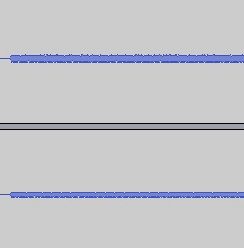
\includegraphics[width=150px]{img/125kHz_TGLS.png}
  \caption{Tarpausinis garso lygio skirtumas esant 125 kHz dažniui, kai garso šaltinio kampas manekeno galvos atžvilgiu siekia 90$^\circ$}
  \label{fig:125kHz_TGLS}
\end{figure}

\begin{figure}[!h]
  \centering
  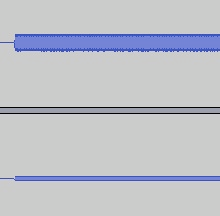
\includegraphics[width=150px]{img/1000kHz_TGLS.png}
  \caption{Tarpausinis garso lygio skirtumas esant 1 MHz dažniui, kai garso šaltinio kampas manekeno galvos atžvilgiu siekia 90$^\circ$}
  \label{fig:1000kHz_TGLS}
\end{figure}

Iš \ref{fig:125kHz_TGLS} ir \ref{fig:1000kHz_TGLS} pav. matome, jog lyginant du skirtingo dažnio garsus (125 kHz ir 1000 kHz), kai garso bangos kritimo kampas siekia 90$\circ$, susidaro tarpausinio garso lygių skirtumas. Kaip ir buvo minėta, esant aukštesniems nei 1,5 kHz dažniams, tarpausinis laiko skirtumas tampa labai mažas ir tuomet dominuoja tarpausinis garsio lygių skirtumas. Fizikinis šio fenomeno paaiškinimas būtų toks, kad esant aukštesniems dažniams, garso bangos sutankėja ir jų galimybė persilenkti aplink galvą stipriai sumažėja. Esant skirtingiems objektų dydžiams ir skirtingiems garso bangų dažniams, išlieka difrakcinė priklausomybė, bet šiuo atveju tai negalioja, nes naudojama standartinė vidutinio žmogaus galvos dydžio manekeno galva. Be abejo išlieka minimalūs skirtumai, nes kiekvieno žmogaus galva turi savo unikalią formą ir dydį, o tai sukuria skirtingą šešėlinį dažnį, bet galima sakyti, jog šis skirtumas yra nykstamai mažas.

\begin{figure}[!h]
  \centering
  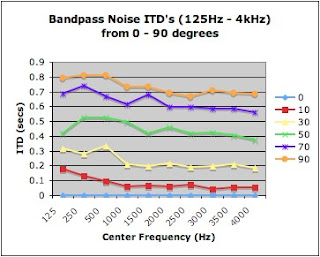
\includegraphics[width=300px]{img/ITD_freq.png}
  \caption{Tarpausinio laiko skirtumo priklausomybė dažnio esant skirtingiems garso bangos kritimo kampams (0$^\circ$ -- 90$^\circ$)}
  \label{fig:ITD_freq}
\end{figure}


\subsection{Kambario impulsinis atsakas}
\label{sect:KIA}

Kambario Impulsinis Atsakas (sutrumpintai \textit{KIA}, angl. \textit{RIR – Room Impulse Response}) – tai yra laiko domeno signalas parodantis dažnių pasiskirstymą ir amplitudės mažėjimą. Naudojant KIA daroma prielaida jog kambario erdvė yra stabili ir linijinė, laikui bėgant nekintanti sistema.

KIA inkapsuliuoja sekančius parametrus:
\begin{enumerate}
  \item Garso signalo vėlinimą (angl. \textit{propagation delay}) – atstumas laike kurį garsas nukeliauja nuo garso šaltinio iki klausytojo.
  \item Tiesioginį garsą (angl. \textit{direct sound}) – tiesioginis garsas atitinką maksimumą kuris nusako trumpiausią atstumą nuo garso šaltinio iki klausytojo.
  \item Ankstyvuosius atspindžius (angl. \textit{early reflections}) – pirmos eilės (dažniausiai atspindį nuo grindų arba lubų), antrosios ir kitų eilių atspindžius.\item Aido liekamąją dalį (angl. \textit{reverberation tail}) – tai stochastinė aido dalis kurioje yra didelis atspindžių kiekis kurie nebegali būti suskirstyti į ankstyvuosius atspindžius.  
  \item Pradinio Vėlinimo Atotrūkis (PVA, angl. \textit{ITDG – Initial Time Delay Gap}) – tai laikas tarp į klausytojo klausos sistemą atvykusio tiesioginio garso ir pirmojo ankstyvojo atspindžio (dažniausiai atsispindėjusio ne nuo grindų). Dažnai norint išvengti papildomų skaičiavimų paprastas signalo vėlinimas yra panaudojamas PVA imituoti.
\end{enumerate}

Šiame darbe yra panaudotas supaprastintas KIA modelis, darant prielaidą jog garso bangą sudaro baigtinis skaičius spindulių sklindančių tiesia linija visomis kryptimis. Ši prielaida yra klaidinga tačiau tokiu būdu yra ženkliai sumažinamas skaičiavimų kiekis kas savo ruožtu leidžia taikyti KIA modelį realiuoju laiku veikiančiame įrenginyje neturinčiame ypač didelių skaičiavimo galimybių. Priešingu atveju nepriėmus anksčiau minėtos prielaidos KIA generavimas tampa labai sudėtingas ir negali būti taikomas realaus laiko binauralinio garso generavimui.


\subsection{Skyriaus apibendrinimas}

Šiame skyriuje buvo paminėti pagrindiniai metodai susiję su binauraliniu garsu. Minimaliam binauraliniam efektui gauti pakanka tik \textit{HRTF} filtrų, bet kaip patvirtina atlikti bandymai -- šis efektas nėra labai įtikinantis ir natūralus. Tačiau jei prieš panaudojant \textit{HRTF} funkcijas garso signale yra užkoduojama kambario akustinė informacija, binauralinio garso efektas tampa panašesnis į realiame pasaulyje susidarančius garsus. 
Darbo metu sukurta garso apdorojimo sistema išnaudoja šiame skyriuje aprašytus metodus sukuriant pakankamai įtikinantį binauralinį efektą.

\section{Sistemos kūrimas}

Šiame skyriuje bus aptartas sistemos kūrimas, bendra struktūros apžvalga bei aprašyti naudojami algoritmai. Pagrindinis dėmesys bus skirtas galvos orientacijos įrenginio daviklių duomenų suliejimo algoritmų bei garso binauralinio garso generavimo metodų aprašymui.

\subsection{Sistemos struktūrinė schema}

\begin{figure}[!h]
  \centering
  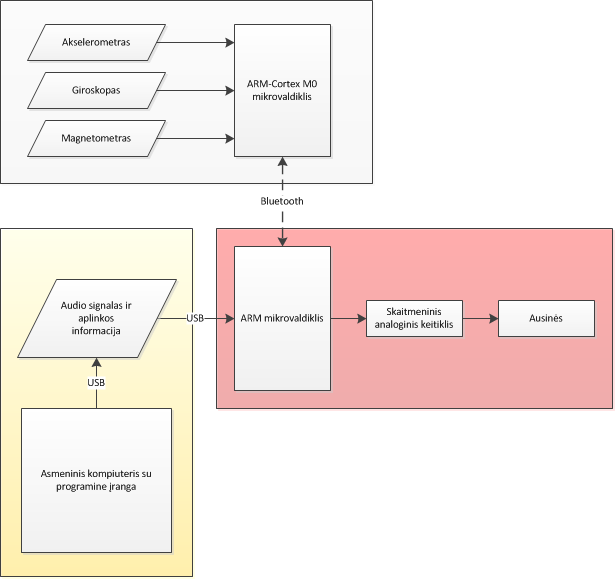
\includegraphics[width=300px]{img/schema.png}
  \caption{Struktūrinė schema}
  \label{fig:full_schematic}
\end{figure}

\ref{fig:full_schematic} pav. pavaizduota baigiamojo bakalaurinio darbo struktūrinė schema. Sistemą sudaro trys dalys:

\begin{itemize}
\item Galvos sekimo įrenginys
\item Garso apdorojimo įrenginys
\item Asmeninis kompiuteris su specializuota programine įranga.
\end{itemize}

Galvos sekimo įrenginys skirtas sekti vartotojo galvos orientacijai erdvėje, tam kad, sistemai suteikti generuojamo garso priklausomybę nuo galvos orientacijos. Ši priklausomybė yra būtina norint kuo tiksliau sugeneruoti binauralinį garsą. Norint įgyvendinti nepriekaištingą galvos sekimo įrenginio veikimą, buvo suprojektuota ir pagaminta spausdintinė plokštė, atitinkanti fizinių išmatavimų ir elektros energijos sąnaudų reikalavimus. Taip pat parašytos dvi programinės įrangos – pačiam galvos orientacijos sekimo įrenginiui bei asmeniniam kompiuteriui. Įrenginio programinė įranga skirta nuskaityti parodymus iš skirtingų jutiklių – akselerometro, magnetometro ir giroskopo, o taipogi juos siųsti į asmeninį kompiuterį tolimesniam apdorojimui. Savo ruoštu, asmeninis kompiuteris su savo programine įranga šiuos duomenis toliau apdoroja. Šiuo atveju atliekama visų daviklių duomenų filtracija ir sujungimas. Tokiu būdu išgaunama galvos orientacija trimatėje erdvėje.

Garso apdorojimo įrenginys – tai baigiamojo bakalaurinio darbo metu sukurta įterptinė sistema skirta binauralinio garso generavimui, joje apdorojami virtualios erdvės akustiniai ypatumai, o taip pat iš asmeninio kompiuterio gautas monofoninis garsas priklausomai nuo galvos sekimo įrenginio surinktų duomenų atitinkamai pakeičiamas. Šių veiksmų visuma sukuria binauralinį efektą. Tad kaip yra matoma iš paveikslo 4.1 pagrindinė sistemos dalis yra garso apdorojimo įrenginys, tačiau neturint tiek virtualios, tiek realios aplinkos duomenų tikrą binauralinį efektą sukurti neįmanoma. Garso apdorojimo įrenginys susideda iš kelių dalių – galingas 32 bitų ARM serijos mikrovaldiklis su integruotu skaitmeninių signalų apdorojimo moduliu, maitinimo stabilizatoriaus, sąsajų bei skaitmeninio – analoginio keitiklio. Pastarasis skirtas skaitmeninį apdorotą signalą paversti į analoginį garso toną. 

\subsection{Jutiklių duomenų sintezės filtras}

Sensor fusion algoritmas yra naudojamas galvos orientacijos nuskaitymo įrenginyje. Galvos orientaciją erdvėje nuskaito trys davikliai: 

triašis akselerometras – pagreičiui kiekvienoje ašyje nustatyti.
\begin{itemize}
\item triašis magnetometras – nustatyti kampą žemės magnetinių linijų ir magnetometro atžvilgiu.
\item Triašis giroskopas – kampiniam pagreičiui trijose ašyse nustatyti.
\end{itemize}

Visi šie trys davikliai turi savo stipriąsias ir silpnąsias puses, tačiau sensor fusion algoritmai padeda padidinti galutinių duomenų tikslumą. Dažniausiai naudojamas filtras – Kalmano, tačiau dėl didelio matematinio skaičiavimo kiekio (kuris neigiamai įtakoja bendrą mažos galios įterptinės sistemos greitaveiką) šiame darbe buvo pasirinktas paprastesnis Madgwick sensor fusion filtras. Palyginus su Kalmano filtru, Madgwicko filtras turi tik vieną žingsnį per kurį yra apskaičiuojami galutiniai duomenis, atsisakius nuspėjimo ir korekcijos žingsnių (kurie naudojami Kalmano filtre) sutaupomas laikas, ko pasėkoje padidėja greitaveika. Tačiau atsisakius prieš tai minėtų dviejų žingsnių suprastėja filtro savybės, nes neatsižvelgiama į prieš tai buvusius duomenis.

Madgwicko filtre orientacijai nusakyti naudojami kvaternionai\footnote{Kvaternionas (lot. \textit{quattor} – keturi) – skaičių aibė, nekomutatyvus kompleksinių skaičių aibės praplėtimas. }, tokiu būdu išvengiamas ašių užsiblokavimo (angl. \textit{gimbal lock}) efektas. Kvaternionas savo paprasčiausioje formoje aprašomas formule \ref{quaterion_1}, kur $r_{x}$, $r_{y}$, $r_{z}$ yra vektoriaus $r$ kampų reikšmės, $\theta$ – pasukimo kampas, $q_{w}$, $q_{x}$, $q_{y}$, $q_{z}$ – kvaterniono $w$, $x$, $y$, $z$ dedamosios. 

\begin{equation}
_{B}^{A}\hat{q}= \begin{bmatrix} q_{1} & q_{2} & q_{3} & q_{4}
\end{bmatrix} = \begin{bmatrix}
\cos\frac{\theta}{2} & -r_{x}\sin\frac{\theta}{2} & -r_{y}\sin\frac{\theta}{2} & -r_{z}\sin\frac{\theta}{2}
\end{bmatrix}
\label{quaterion_1}
\end{equation}

\begin{figure}[!h]
  \centering
  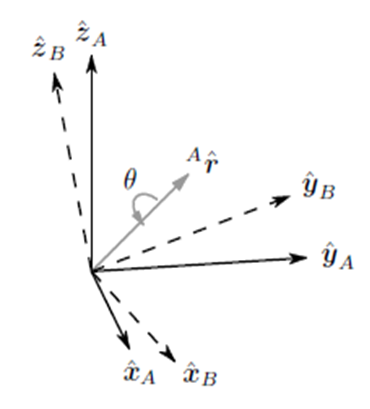
\includegraphics[width=150px]{img/quaternion_frame.png}
  \caption{Dviejų rėmų orientacijos kitimas vienas kito atžvilgiu.}
  \label{fig:quaternion_2}
\end{figure}

Paveikslas \ref{fig:quaternion_2} nusako rėmo\footnote{Geometrijoje objekto (linijos, plokštumos ar kietojo kūno) orientacija erdvėje yra dažnai pateikiama kaip vieno rėmo orientacija kito rėmo atžvilgiu, tokiu atveju pirmasis rėmas vadinamas atskaitos rėmu (angl. \textit{frame of referrence})} (angl. \textit{frame}) B orientaciją, jį pasukus kampu $\theta$ pagal $A_{\hat{r}}$  ašį, kai pradinė rėmo B orientacija buvo sutapusi su rėmo A orientacija.

\begin{equation}
_{B}^{A}R = \begin{bmatrix} 
   2q_{w}^{2} - 1 + 2q_{x}^{2} & 2(q_{x}q_{y}+q_{w}q_{z}) & 2(q_{x}q_{z}+q_{w}q_{y})
\\ 2(q_{x}q_{y}-q_{w}q_{z}) & 2q_{w}^{2} - 1 + 2q_{y}^{2} & 2(q_{y}q_{z}+q_{w}q_{x})
\\ 2(q_{x}q_{z}+q_{w}q_{y}) & 2(q_{y}q_{z}-q_{w}q_{x}) & 2q_{w}^{2} - 1 + 2q_{y}^{2}
\end{bmatrix}
\label{equ:rotation_matrix}
\end{equation}

Taipogi kvaternioną galima išreikšti pasukimo matricos pavidalu \ref{equ:rotation_matrix}, tai suteikia lankstumo skaičiuojant pasisukimą.

Matricinė kvaterniono išraiška labai patogi norint orientaciją paversti Eulerio sistemos kampais arba atliekant operacijas susijusias su kampais. Tačiau saugoti orientacijos informaciją tokiu pavidalu nėra patogu dėl anksčiau minėto ašių užsiblokavimo. 

Kaip matoma iš paveikslo \ref{fig:quaternion_2} apskaičiuot kvaternionams reikalingi du rėmai, pirmasis atskaitos rėmas (angl. \textit{reference frame}) antrasis -- sistemos rėmas. Šiame darbe rėmu A (atskaitos rėmas) bus laikoma žemė, o rėmas B – galvos orientacijos įrenginys (sistemos rėmas).

\begin{figure}[htbp]
  \centering
  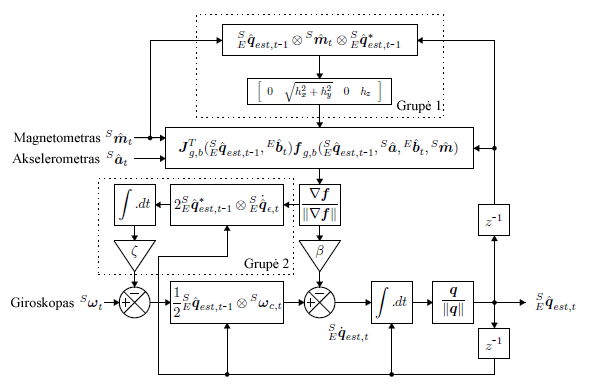
\includegraphics[width=390px]{img/madgwick.png}
  \caption{Madgwicko filtro schema}
  \label{fig:madgwick}
\end{figure}

Bendra filtro schema pavaizduota \ref{fig:madgwick} pav. Kur $^{S}\hat{m}_{t}$ magnetometro duomenys, $^{S}\hat{a}_{t}$ – akselerometro, $^{S}\hat{\omega}_{t}$  – giroskopo parodymai. \ref{fig:madgwick} pav. parodo pilnąjį Madgwicko filtrą MARG (angl. \textit{Magnetic, Angular Rate, and Gravity}) sistemai. Grupė 1 skirta pašalinti magnetometro magnetinius triukšmus (angl. \textit{Magnetic distortion}), Grupė 2 – skirta pasinaudojant akselerometro ir magnetometro duomenimis sumažinti giroskopo dreifą. Tokiu būdu filtras įgauna magnetometro triukšmo ir giroskopo dreifo kompensavimo savybes. Filtro rezultatas – $_{E}^{S}\hat{q}_{est,t}$ pilna objekto orientacija žemės atžvilgiu išreikšta kvaternionu. 

\subsection{Garso apdorojimo mechanizmas}

Garso apdorojimo įrenginio programinę įrangą sudaro dvi dalys – programinė įranga asmeniniame kompiuteryje bei programinė įranga esanti pačiame garso apdorojimo įrenginyje. Norint įgyvendinti aparatinio lygmens garso išvestį, visų pirma, reikia skaitmeninio garso duomenų bei aparatinės įrangos skirtos skaitmeninį garsą paversti į analoginį (SAK – skaitmeninis analoginis keitiklis). Skaitmeninio garso informacija bei duomenys siunčiami naudojant \textit{RS232} protokolą. Šių duomenų šaltinis – asmeninis kompiuteris su savo programine įranga. Skaitmeninio garso duomenų siuntimui į SAK naudojamas \textit{I2S} protokolas. \textit{I2S} – tai nuoseklusis duomenų perdavimo protokolas, kuris buvo sukurtas sujungti skaitmeninio garso įrenginius tarpusavyje. Jis plačiai taikomas garso atkūrimo ir įrašymo pramonėje (\textit{blue-ray}, \textit{CD}, \textit{DVD} grotuvuose ir kt.). Dažniausiai protokolas naudojamas sujungus tam tikro formato dekoderius ir skaitmeninius-analoginius keitiklius tarpusavyje. Protokolo fizinis lygmuo susideda iš trijų linijų – valdančioji bitų perdavimo dažnio linija, kanalo pasirinkimo linija bei duomenų perdavimo linija. Duomenys šiuo protokolu siunčiami sinchroniniu būdu. T.y. duomenys nuskaitomi tik esant aukštam valdančiosios bitų perdavimo linijos įtampos lygiui. Kanalo parinkimas (kairiojo ar dešiniojo) vyksta keičiant kanalo parinkimo linijos įtampos lygį. Šis keitimas privalo būti atliktas prieš perduodant paskutinį esamojo kanalo duomenų bitą. \ref{fig:garso_apdorojimas} pav pavaizduotas garso apdorojimo įrenginio programos algoritmo blokinė diagrama.

\begin{figure}[!ht]
  \centering
  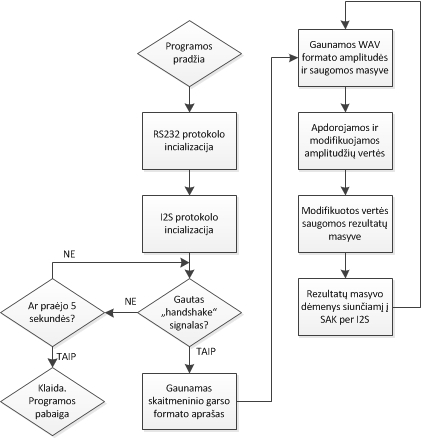
\includegraphics[width=400px]{img/garso_apdorojimas.png}
  \caption{Garso apdorojimo įrenginio programos algoritmo blokinė diagrama}
  \label{fig:garso_apdorojimas}
\end{figure}

Kaip matoma iš \ref{fig:garso_apdorojimas} pav., programos algoritmas prasideda nuo \textit{RS232} bei \textit{I2S} protokolų įgalinimo. \textit{STM32F407-VGT}, kaip ir 8 bitų \textit{AVR} mikrovaldiklis, turi aparatinio lygmens \textit{RS232} protokolą. Pastarajame naudojamas 8N1 standartas – 8 duomenų perdavimo bitai, 1 start bitas, 1 stop bitas ir jokio lyginumo bito. Kaip ir buvo minėta anksčiau, skaitmeninio garso duomenų perdavimui naudojamas \textit{I2S} protokolas. Pasirinktas 32 bitų mikrovaldiklis turi aparatinio lygmens \textit{I2S} protokolą. Taigi, norint įgalinti protokolą, reikia įrašyti tam tiukras vertes į atitinkamus registrus programiškai. Toliau programos algoritme seka „handshake“ signalas. Tai tam tikras sutartinis „pasisveikinimo“ signalas siunčiamas \textit{RS232} protokolu asmeniniam kompiuteriui. Jeigu gaunamas teigiamas atsakymas, tuomet algoritmas tęsiamas. Jei negaunamas joks atsakymas, tikrinama ar praėjo 5 sekundės nuo „pasisveikinimo“ signalo išsiuntimo. Jei minėtasis laikas praėjo, tuomet registruojama programos algoritmo klaida ir programa yra užbaigiama. Jei 5 sekundės nepraėjo, tuomet toliau laukiamas atsakymas. Jei sulaukiamas „pasisveikinimo“ patvirtinimas, tuomet tęsiamas programos algoritmas. Tolimesnė programos eiga – gaunamas skaitmeninio garso duomenų aprašas. Pavyzdžiui – 16 bit duomenys vienam kanalui, 44,1 kHz diskretizavimo dažnis. Gavus šį aprašą, sukonfigūruojamos garso išvesties funkcijos pagal gautą formatą. Toliau programa pereina prie begalinio ciklo, kuriame vyksta visos likusios operacijos galutiniam garso išvedimui į ausines. Visų pirma, per \textit{RS232} sąsają gaunamos \textit{WAV} failo amplitudžių vertės. Sekančiame žingsnyje vyksta visos apdorojimo bei modifikavimo, pagal esamą žmogaus galvos orientaciją, operacijos. \textit{Matlab} kodo fragmente \ref{code:conv_sound} pateiktas pavizdys, kaip sąsukos būdu yra kodifikuojamas garsas. Visos modifikuotos amplitudžių vertės paruošiamos galutiniam panaudojimui ir saugomos rezultatų masyve. Vertės iš rezultatų masyvo paeiliui siunčiamos į skaitmeninį-analoginį keitiklį \textit{I2S} protokolui.

\begin{cfigure}
  \centering
  \caption{Sąsukos taikymas garso apdorojimo įrenginyje. \textit{Matlab} kodo fragmentas}
  \label{code:conv_sound}
  \lstinputlisting{sources/conv.m}
\end{cfigure}

\newpage

\subsection{Galvos sekimo įrenginys}

Šiame poskyryje aptariamas galvos sekimo įrenginio programos algoritmas. \ref{fig:head_tracker} paveiksle pavaizduota algoritmo blokinė schema.

\begin{figure}[!ht]
  \centering
  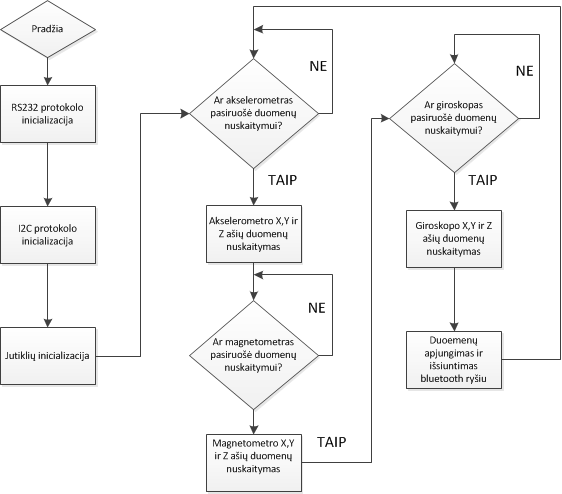
\includegraphics[width=400px]{img/head_tracker.png}
  \caption{Galvos sekimo įrenginio programos algoritmo blokinė diagrama}
  \label{fig:head_tracker}
\end{figure}

Kaip matome iš \ref{fig:head_tracker} paveikslo, programos kodo pradžioje vyksta kintamųjų sukūrimas bei naudojamų įėjimų/išėjimų nustatymas. Kadangi naudojamų jutiklių duomenų perdavimo standartinis protokolas yra \textit{I2C}, todėl reikia įgyvendinti \textit{I2C} protokolo nustatymo mikrovaldiklyje operacijas. Pasirinktas mikrovaldiklis \textit{Atmel Atmega8} savyje turi aparatinio lygio \textit{I2C} valdymo bloką. Pagal specifikacinį \textit{AVR} mikrovaldiklio aprašą, norint įgalinti \textit{I2C} protokolą, reikia nustatyti duomenų perdavimo dažnį. Pasirinktas dažnis – 400 kHz. Tolimesnis programos kodas – tai jutiklių pradinių parametrų nustatymas. Norint panaudoti \textit{bluetooth} duomenų perdavimo ryšį, naudojamas \textit{UART} protokolas. \textit{Atmega8} mirkovaldiklis taip pat turi aparatinio lygio \textit{UART} protokolo bloką. Taigi tinkamam pastarojo veikimui, reikia jį įgalinti programiškai kaip ir \textit{I2C} protokolą. Pasirinkta duomenų perdavimo sparta – 57600 bodų per sekundę.
Giroskopo \textit{L3G4200D} pradiniai nustatymai:

\begin{itemize}
\item Energijos taupymo režimo išjungimas. T.y. jutiklio įjungimas
Magnetometro \textit{LSM303DLH} pradiniai nustatymai:
\item Parenkamas duomenų atnaujinimo dažnis – 75 Hz
\item Parenkamas ±2,5 Gauss įėjimo diapazonas
\item Parenkamas nenutrūkstantis duomenų atnaujinimas
\end{itemize}

Akselerometro \textit{LSM303DLH} pradiniai nustatymai:
\begin{itemize}
\item Parenkamas 1000 Hz duomenų atnaujinimo dažnis
\item Išjungiamas energijos taupymo veikimo režimas.
\item Išjungiamas vidinis duomenų filtras 
\item Nustatomas duomenų eiliškumas 8 bitų registruose
\end{itemize}

Atlikus jutiklių parametrų nustatymus, programos algoritmas pereina prie begalinio ciklo jutiklių duomenų nuskaitymui ir persiuntimui per \textit{bluetooth} ryšį. Duomenys nuskaitomi iš kiekvieno jutiklio šia eilės tvarka: akselerometro, magnetometro bei giroskopo duomenų nuskaitymas. Prieš kiekvieno jutiklio duomenų nuskaitymą yra laukiamas patvirtinimas, jog jutiklis yra pasirengęs perduoti duomenis. Todėl tikslaus duomenų atnaujinimo dažnio nustayti neįmanoma, nes kiekvieną ciklo iteraciją jutiklių pasirengimas perduoti duomenis gali skirtis. Per kiekvieną begalinio ciklo iteraciją nuskaitomos visos 3 jutiklių ašys – $X$,$Y$,$Z$. Kadangi pastarieji yra padidinto tikslumo (12 bitų), tai nuskaitant duomenis 8 bitų mikrovaldikliu \textit{I2C} protokolu, šiuos duomenis reikia apdoroti. Taip yra todėl, kad tiek jutiklių, tiek mikrovaldiklio registrai yra 8 bitų, bei \textit{I2C} protokolas perduoda tik 8 bitus duomenų vienos užklausos metu. Duomenų sujungimas šiuos atveju, tai tiesiog 8 aukščiausiųjų bitų perstūmimas į kairę lyginant su žemiausiais 8 bitais. Taip gaunamas 12 bitų tikslumas. Visi jutiklių duomenys po vienos ciklo iteracijos apjungiami į vieną string formato eilutę ir išsiunčiami bluetooth ryšiu, naudojant \textit{UART} protokolą.

\subsection{Binaurainio garso efekto mechanizmo algoritmas}

\ref{fig:binaural_schem} pav. iliustruoja sukurtą mechanizmą binauraliniam garsui generuoti. Kaip matoma iš \ref{fig:binaural_schem} pav. pateiktos schemos, pirmasis žingsnis turint originalaus garso duomenis yra apskaičiuoti KIA abiems ausims. Pagal gautą KIA funkciją sąsukos veiksmu modifikuojamas originalus garsas. Įvykdžius šį žingsnį vieno kanalo garsas tampa dvikanaliu. Gautas tarpinis garso signalas sujungiamas su parinktu HRTF filtru. Po šio žingsnio gaunamas binauralinis garso signalas.

\begin{figure}[!ht]
  \centering
  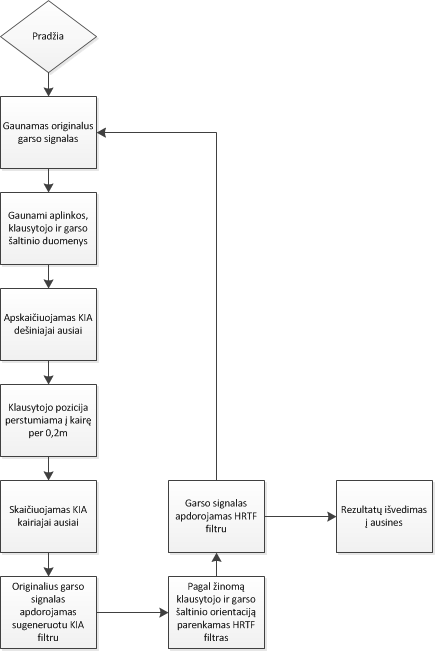
\includegraphics[width=300px]{img/binaural_schem.png}
  \caption{Galvos sekimo įrenginio programos algoritmo blokinė diagrama}
  \label{fig:binaural_schem}
\end{figure}

\subsection{KIA generavimas}

Žemiau yra pateikta \textit{Matlab} funkcija generuoti kambario impulsiniam atsakui pasinaudojus skyriuje \ref{sect:naudojami_metodai} aprašyta teorine dalimi bei \ref{sect:KIA} poskyryje išsakytomis prielaidomis.
Pasinaudojant Stepheno G. McGoverno straipsnyje „A Model for Room Acoustics“ aprašytomis formulėmis galima sukurti paprastą kambario impulsinio atsako filtrą.
\ref{equ:virtual_sounds} formulė padeda rasti virtualaus šaltinio (garso atspindžio) poziciją $x$ ašyje. 

\begin{equation}
x_{i}=(-1)^{i}x_{S}+\left[ i+\frac{1-(-1)^{i}}{2}\right] x_{r}
\label{equ:virtual_sounds}
\end{equation}

čia $x_{S}$ – tikrojo garso šaltinio x koordinatė, $x_{r}$ – kambario ilgis, $i$ – virtualaus garso šaltinio (atspindžio) eilės numeris. Atėmus iš virtualaus šaltinio $x$ koordinatės klausytojo taško $x$ koordinatę galima rasti atstumą $x$ ašyje tarp klausytojo ir virtualaus šaltisnio. Tai aprašo formulė \ref{equ:dist_x}, toliau sekančios formulės 4.5 ir 4.6 aprašo atstumą tarp klausytojo ir garso šaltinio $y$ ir $z$ ašyse atitinkamai:

\begin{equation}
x_{i}=(-1)^{i}x_{S}+\left[ i+\frac{1-(-1)^{i}}{2}\right] x_{r}-x_{m}
\label{equ:dist_x}
\end{equation}

\begin{equation}
x_{i}=(-1)^{i}x_{S}+\left[ i+\frac{1-(-1)^{i}}{2}\right] y_{r}-y_{m}
\label{equ:dist_y}
\end{equation}

\begin{equation}
x_{i}=(-1)^{i}x_{S}+\left[ i+\frac{1-(-1)^{i}}{2}\right] z_{r}-z_{m}
\label{equ:dist_z}
\end{equation}

Rasti pilną atstumą kiekvienam virtualiam garso šaltiniui galima pasinaudojus Pitagoro teorema \ref{equ:pitagor} 

\begin{equation}
d_{ijk}=\sqrt{x_{i}^{2}+y_{i}^{2}+z_{i}^{2}}
\label{equ:pitagor}
\end{equation}

Toliau norint rasti kambario impulsinį atsaką reikia išsivesti vieneto impulsinio atsako funkciją  (angl. \textit{unit impulse response function}). Padalinus \ref{equ:pitagor} formulę iš garso greičio ore gaunamas virtualaus garso šaltinio impulsinis atsakas \ref{equ:unit_impulse_resp}.

\begin{equation}
u_{ijk}(t)=\frac{d_{ijk}}{c}
\label{equ:unit_impulse_resp}
\end{equation}

čia $t$ – laikas, $d_{ijk}$ – atstumas gautas iš \ref{equ:pitagor} formulės, $c$ – garso greitis (340.29 m/s), $\frac{d_{ijk}}{c}$ – efektinis kiekvieno atspindžio laiko skirtumas. Pasinaudojus \ref{equ:unit_impulse_resp} formule galima išsivesti ieškomą funkciją \ref{equ:unit_impulse_resp_funct}.

\begin{equation}
a_{ijk}= \left\{
  \begin{array}{l l}
    1 & \quad \text{jeigu $u_{ijk} = 0$}\\
    0 & \quad \text{priešingu atveju}\\
  \end{array} \right.
\label{equ:unit_impulse_resp_funct}
\end{equation}

Šiame žingsnyje gaunama aibė atspindžių kurioje kiekvienas atspindys turi impulsą lygu 1, kai $u_{ijk}=0$. Tikrasis garso bangos impulsas mažėja priklausomai nuo atstumo tarp šaltinio ir kliūčių pakeliui. Sekantys žingsniai ištaiso šią problemą. Garso impulsas yra atvirkščiai proporcingas atstumui tarp garso šaltinio ir klausytojo \ref{equ:unit_impulse_resp_corrected}.

\begin{equation}
b_{ijk}	\sim\frac{1}{d_{ijk}}
\label{equ:unit_impulse_resp_corrected}
\end{equation}

Kitas svarbus parametras yra garso atspindžio atsispindėjimų skaičius. Jei visų sienų atspindžių koeficientai vienodi, galima paimti atspindžio koeficientą $r_{w}$ keliant laipsniu $n$, kur $n$ yra bendras atspindžių skaičius gauname $n=|i|+|j|+|k|$. Taigi atsispindėjimų skaičiui apskaičiuoti taikytina formulė \ref{equ:atspindziu_sk}:

\begin{equation}
r_{ijk}	= r_{w}^{|i|+|j|+|k|}
\label{equ:atspindziu_sk}
\end{equation}

Taigi kad gauti pilnąjį signalo impulsą, reikia sudauginti \ref{equ:unit_impulse_resp_corrected} ir \ref{equ:atspindziu_sk} formules, taip gaunama formulė \ref{equ:full_impulse}).

\begin{equation}
e_{ijk}	= b_{ijk} r_{ijk}
\label{equ:full_impulse}
\end{equation}

Paskutinis žingsnis kambario impulsinio atsako skaičiavime yra sumavimas pagal \ref{equ:RIA_sum} formulę:

\begin{equation}
h(t) = \sum_{i=-n}^{n}\sum_{j=-n}^{n}\sum_{k=-n}^{n} a_{ijk} e_{ijk}
\label{equ:RIA_sum}
\end{equation}

Pateiktas \textit{Matlab} paketo išeities kodo fragmentas \ref{code:RIA_gen} skirtas generuoti šiame poskyryje aprašytą kambario impulsinį atsaką.

\begin{cfigure}
  \centering
  \caption{KIA generavimo \textit{Matlab} funkcija}
  \label{code:RIA_gen}
  \lstinputlisting{sources/RIA.m}
\end{cfigure}

\newpage
\subsection{Realios sistemos specifikacija}

Šiame poskyryje bus aptartas ir aprašytas realus įrenginys pagrįstas ankščiau aprašytomis teorijomis. Reali sistema susideda iš programines ir elektronikos dalių.

\ref{fig:headtracker_schematic} paveiksle matoma galvos orientacijos sekimo įrenginio mikrovaldiklinė dalis. Įrenginiui valdyti panaudotas 8 bitų mikrovaldiklis \textit{ATMEL ATMEGA8 TQFP32} korpuse. Šioje įrenginio schemos dalyje matomas pats mikrovaldiklis, programavimo sąsaja bei išvesties jungtys. Taktinis mikrovaldiklio darbo dažnis – 16 MHz.

\begin{figure}[htbp]
  \centering
  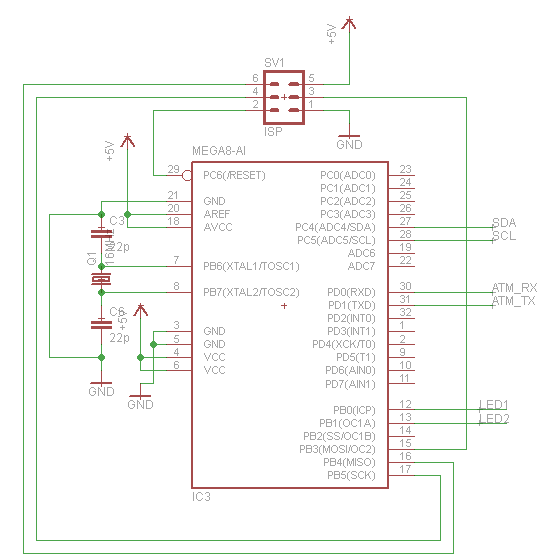
\includegraphics[width=390px]{img/headtracker_schematic.png}
  \caption{Galvos orientacijos sekimo įrenginio elektrinės – principinės schemos mikrovaldiklio dalis}
  \label{fig:headtracker_schematic}
\end{figure}

Tai yra maksimalus įmanomas (teorinis) \textit{ATMEGA8} taktinis darbo dažnis. Šį dažnį generuoja kvarcinis rezonatorius, o pastarojo darbo stabilumui palaikyti naudojami mažos talpos kondensatoriai jungiami nuosekliai su kvarciniu rezonatoriumi ir įžeminimu. Išvesties jungtys \textit{ATM\_RX} ir \textit{ATM\_TX} naudojamos kaip \textit{RS232} sąsaja su \textit{Bluetooth} moduliu. \textit{SDA} ir \textit{SCL} – \textit{I2C}  sąsaja su jutiklių spausdintine plokšte.

\begin{figure}[htbp]
  \centering
  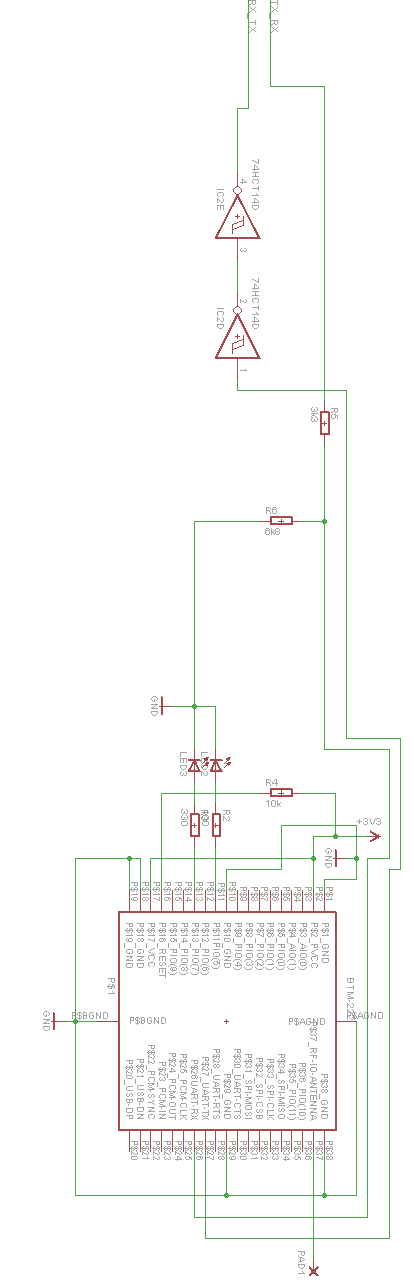
\includegraphics[width=200px]{img/head_tracker_sender.png}
  \caption{Galvos orientacijos sekimo įrenginio elektrinės – principinės schemos siųstuvinė-imtuvinė dalis}
  \label{fig:headtracker_sender}
\end{figure}

\ref{fig:headtracker_sender} paveiklėlyje matome galvos orientacijos sekimo įrenginio siųstuvinę-imtuvinę dalį, kurią sudaro \textit{Bluetooth} modulis \textit{BTM-222}, Šmito trigeris bei įtampų daliklis R5-R6. Pats \textit{BTM-222} modulis veikia per \textit{RS232} sąsają, todėl juo naudotis gana paprasta. Šmito trigeris čia naudojamas dėl tos pačios priežasties, kaip ir įtampų daliklis – suderinti skirtingus loginių įtampų lygius. Kadangi mikrovaldiklis veikia naudojant 5 V maitinimą, o Bluetooth modulis – 3,3 V, taigi norint šiems dviems įrenginiams keistis duomenimis, reikalinga suderinti skirtingus įtampų lygius. Kai duomenys siunčiami iš mikrovaldiklio (su 5 V loginiais lygiais), tai 3,3 V loginį lygį užtikrina įtampų daliklis R5-R6. Duomenims keliaujant priešinga linkme, įtampų lygių suderinamumą užtikrina Šmito trigeris.

\begin{figure}[htbp]
  \centering
  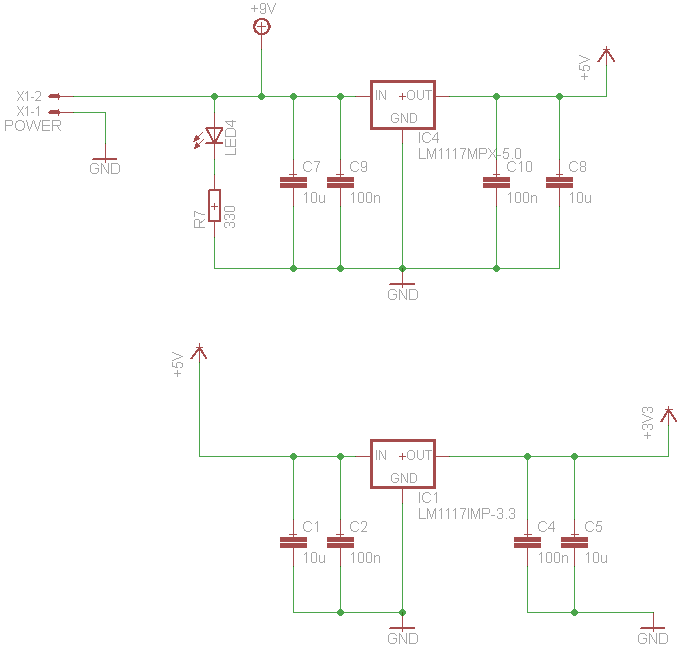
\includegraphics[width=390px]{img/head_tracker_stabilizer.png}
  \caption{Galvos orientacijos sekimo įrenginio elektrinės – principinės schemos maitinimo įtampos stabilizavimo dalis}
  \label{fig:headtracker_stabilizer}
\end{figure}

\ref{fig:headtracker_stabilizer} pav. matoma galvos orientacijos sekimo įrenginio maitinimo šaltinio principinė – elektrinė schema. Ji susideda iš dviejų įtampos stabilizatorių:  \textit{LM1117MPX-5.0} bei \textit{LM1117IMP-3.3}. Abi stabilizatoriai stabilizuoja įėjimo įtampą atitinkamai – 5 V ir 3.3 V. Nepriekaištingam jų veikimui reikalingi filtro kondensatoriai jungiami lygiagrečiai su neigiamu šaltinio poliumi tiek prieš reguliatorius tiek už jų. Įtampos stabilumas ypatingai svarbus žinant, jog mikrovaldiklis dirba gana aukštu dažniu – 16 MHz. Kaip ir buvo minėta anksčiau, 5 V maitinimo įtampa naudojama mikrovaldiklio daliai, o 3.3 V – \textit{Bluetooth} moduliui.

\begin{figure}[htbp]
  \centering
  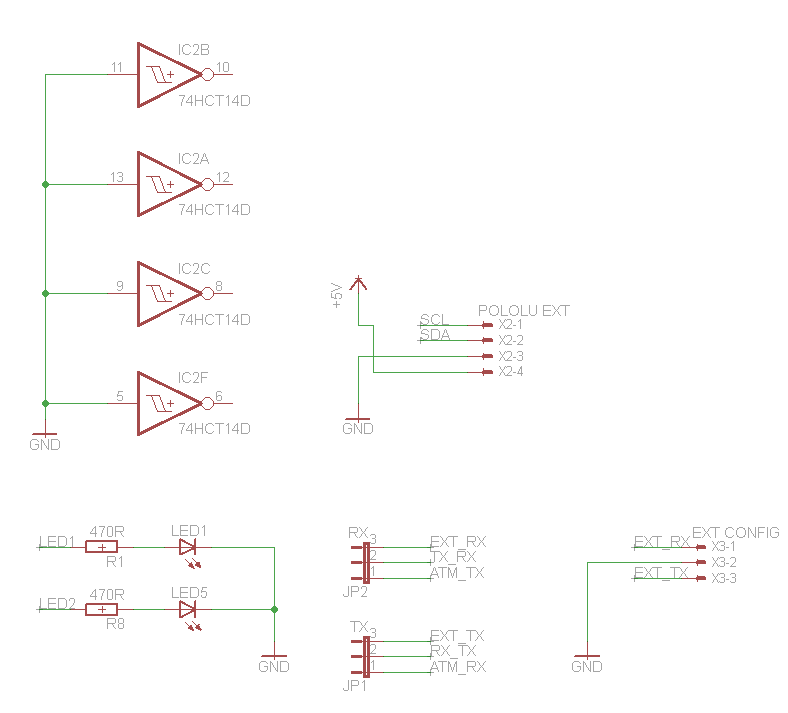
\includegraphics[width=390px]{img/head_tracker_links.png}
  \caption{Galvos orientacijos sekimo įrenginio elektrinės principinės schemos fizinių sąsąjų dalis}
  \label{fig:headtracker_links}
\end{figure}

\ref{fig:headtracker_links} pav. pavaizduotos schemos dalyje matomos fizinės išvesties-įvesties jungtys bei Šmito trigerio mikroschemos nepanaudotų kojelių pajungimas į žemę. Pastarasis veiksmas atliekamas, nes taip pataria specifikacinis mikroschemos aprašas. \textit{POLOLU EXT} jungtis atsako už mikrovaldiklio ir jutiklinės plokščių sujungimą \textit{I2C} sąsaja, bei užtikrina 5 V maitinomo įtampą jutiklinei spausdinintei plokštei. \textit{RX} ir \textit{TX} jungtys – tai trumpikliai, kurie leidžia pasirinkti dvejopą plokštės veikimą – išorinė \textit{RS232} sąsaja skirta klaidų tikrinimui ir \textit{Bluetooth} modulio konfigūravimui. Antras veikimo būdas – mikrovaldiklio tiesioginė sąsaja su \textit{Bluetooth} moduliu. Ir paskutinė jungtis –\textit{EXT. CONFIG} ir yra jungtis skirta vienam iš \textit{RS-232} sąsajos veikimo būdui.

\subsection{Skyriaus apibendrinimas}

Šiame skyriuje buvo pateiktas ir aprašytas sistemos veikimas. Pateiktos blokinės schemos, trumpai aprašytas \textit{Matlab} terpėje sukurtas išeities kodas koncepcijai patikrinti. Realios sistemos specifikacijoje aprašyta sistemos schemotechnika, pademonstruotos ir paaiškintos darbo metu sukurttos plokštės.

\section{Sistemos patikra}

Šiame skyriuje bus aprata sistemos partikra bei jos eiga. Bus bandoma pademonstruoti jog baigiamojo bakalaurinio darbo metu sukurta sistema atitinka jai iškeltus techninius reikalavimus.

\subsection{Galvos sekimo įrenginys}

Šis poskiris skirtas apibendrinti galvos sekimo įrenginio veikimą bei jo charakteristikas.

\subsubsection{Jutiklių duomenų sintezės tikslumo tyrimas}

Didelis dėmesys buvo skirtas jutiklių duomenų sintezei. Algoritmo tiklumas buvo tikrinamas pasitelkiant specialiai paruoštą stalą, tai iliustruoja \ref{fig:headtracker_test1} pav.

\begin{figure}[htbp]
  \centering
  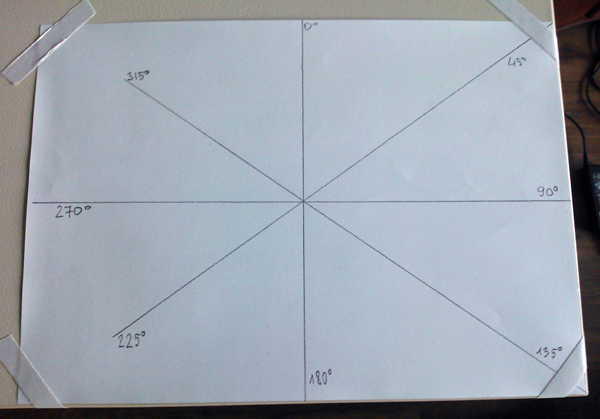
\includegraphics[width=350px]{img/head_tracker_testu_stalas.png}
  \caption{Galvos orientacijos sekimo įrenginio testas}
  \label{fig:headtracker_test1}
\end{figure}

Kaip matoma iš \ref{fig:headtracker_test1} pav. lapas suskirstytas į lygias dalis po 45$^\circ$. Testo pradžioje galvos sekimo įrenginys buvo padėtas ties 0$^\circ$ žyme ir sukalibruotas. kaskart pasukant galvos sekimo įrenginį 45$^\circ$ kampu buvo užfiksuojami jutiklių duomenų sintezės rodmenys, tai iliustruoja \ref{fig:headtracker_test2} pav. Šis testas buvo atliktas po 40 kartų su kiekviena ašimi. Rezultate gauti duomenys parodė pakankamai gerą tikslumą ir toleruotiną paklaidą. Reikia paminėti jog toks testas nėra labai tikslus, tačiau jis leižia padaryti preliminiarias išvadas dėl sistemos tikslumo. Testų rezultatus atspindi \ref{fig:headtracker_test3} grafikas. 

\begin{figure}[htbp]
  \centering
  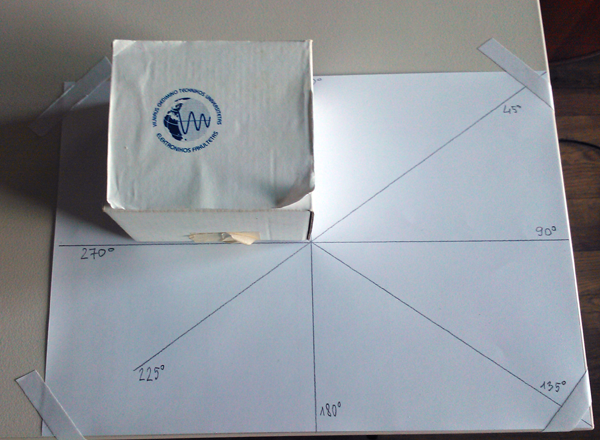
\includegraphics[width=350px]{img/head_tracker_testas.png}
  \caption{Galvos orientacijos sekimo įrenginio testas}
  \label{fig:headtracker_test2}
\end{figure}

\begin{figure}[htbp]
  \centering
  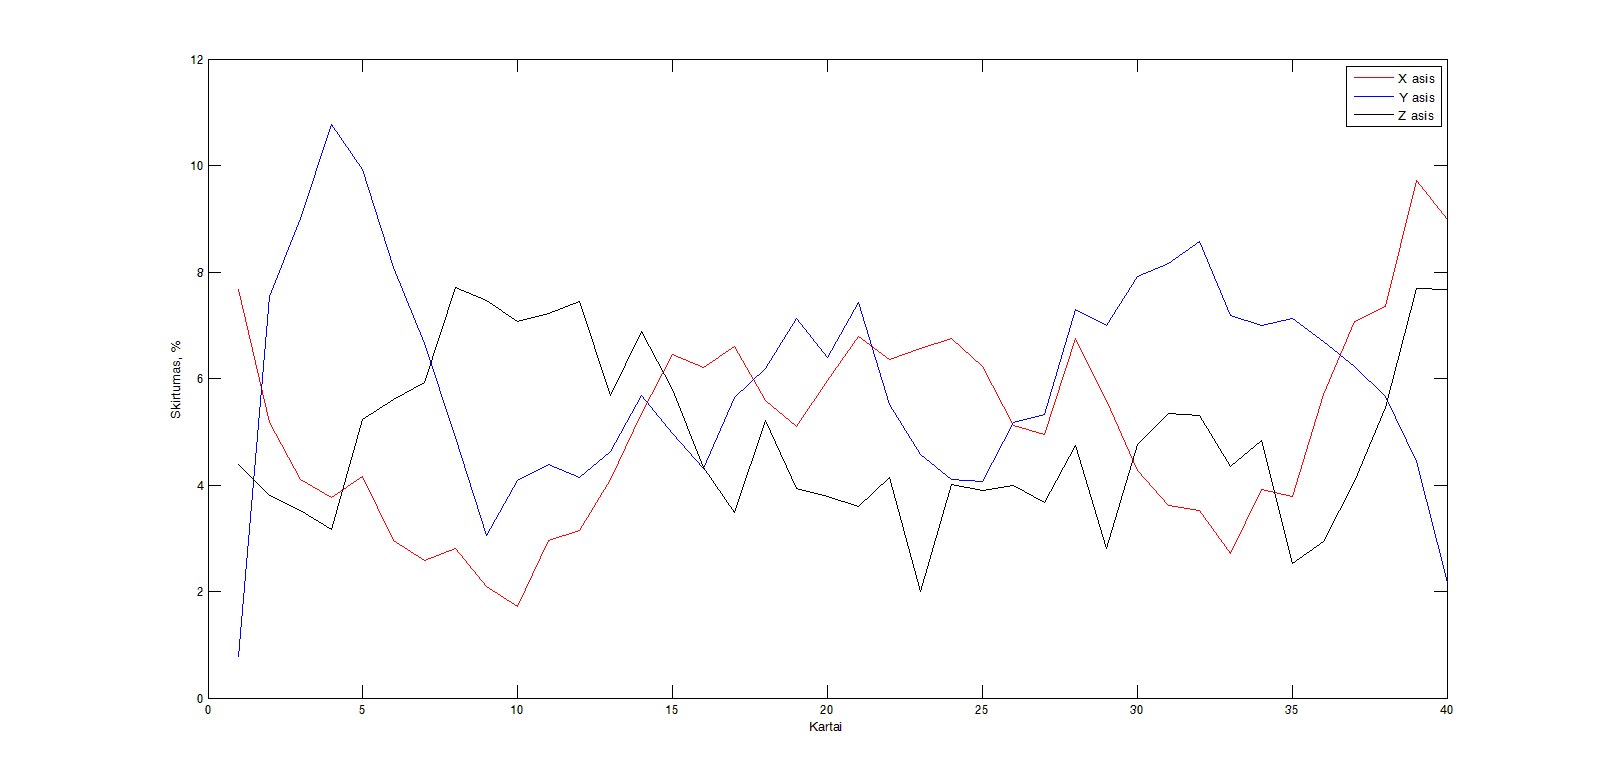
\includegraphics[width=500px]{img/headtracker_axis.png}
  \caption{Galvos orientacijos sekimo įrenginio paklaidų grafikas}
  \label{fig:headtracker_test3}
\end{figure}

Iš \ref{fig:headtracker_test3} grafiko matyti jog paklaida yra labiau atsitiktinio pobūdžio. Didesnę paklaidą galėjo lemti atlikto testo netikslumas

\subsubsection{Energijos suvartojimo patikra}

Patikra buvo atliekama naudojant skaitmeninį oscilografą. Matavimai buvo atliekami įrenginių įjungimo metu du kartus -- šalto paleidimo metu bei po 5 minučių įrenginių veikos. Toks pasirinkimas grindžiamas elektros energijos suvartojimo padidėjimu pakilus darbinei temperatūrai. \ref{fig:headtracker_coldboot} pav. matoma galvos orientacijos sekimo įrenginio elektros srovės suvartojimo priklausomybė nuo laiko šalto paleidimo metu. Kaip ir buvo minėta, matavimai atlikti naudojant skaitmeninį oscilografą. Srovės oscilogramų duomenys, pasirinkta raiška, transformuoti į skaitinių reikšmių lentelę. Šios vertės toliau buvo panaudotos Matlab programos terpėje braižant srovės suvartojimo laikines priklausomybes.

\begin{figure}[htbp]
  \centering
  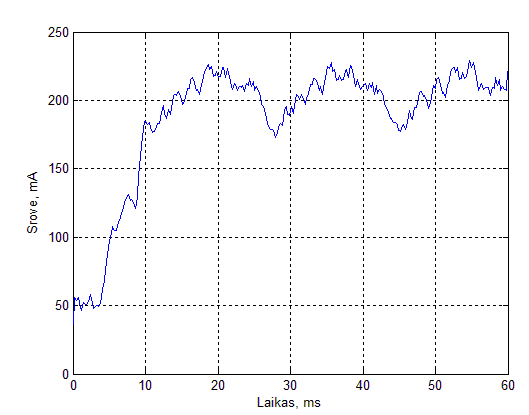
\includegraphics[width=400px]{img/head_tracker_coldboot.png}
  \caption{Galvos orientacijos sekimo įrenginio vartojamos elektros srovės priklausomybė nuo laiko šalto paleidimo metu.}
  \label{fig:headtracker_coldboot}
\end{figure}

Kaip matome iš \ref{fig:headtracker_coldboot} paveikslo, įrenginio paleidimo metu srovė kyla nuo 50 mA iki ~170 mA. Tuo metu vyksta mikrovaldiklio, \textit{bluetooth} modulio kitos periferijos įgalinimas. Tolimesnis srovės suvartojimo svyravimas atsiranda dėl jutiklių duomenų nuskaitymo ir išsiuntimo per bluetooth ryšį naudojant RS232 prievadą. Maksimalus srovės suvartojimas siekia apie 230 mA. Tai yra gana didelė reikšmė, žinant, kad įrenginys yra mobilus ir jo pagrindinis maitinimo šaltinis yra 9 V baterija. Didžiąją dalį srovės suvartoja \textit{bluetooth} modulis ir įtampos stabilizatoriai. Pagal specifikacinį aprašą, \textit{bluetooth} modulio vidutinis srovės suvartojimas siekia net 114 mA. Tai yra net pusė maksimalios suvartojamos elektros srovės. Taigi norint sumažinti bendrą energijos suvartojimą, reikia kiek įmanoma mažinti duomenų atnaujinimo dažnį ir naudoti energijos taupymo režimus. Taip pat didelę dalį energijos suvartojimo sudaro įtampos stabilizatoriai. Ant 5V įtampos stabilizatoriaus atsiranda 4 V įtampos kritimas. Visas šis kritimas išspinduliuojamas šilumine energija į aplinką. Taip prarandamas didelis kiekis elektros energijos. Tai yra visiškai neefektyvu, bet taisytina. Vienas iš būdų – sumažinti elektros energijos maitinimo šaltinio įtampą. Dar vienas įtampos kritimas atsiranda ant 3.3 V įtampos stabilizatoriaus. Kadangi jis jungiamas jau po 5 V įtampos reguliatoriaus, tai atsiradęs kritimas tesiekia 1.7 V. Šioje vietoje sutaupyti energijos neišeina. Vienintelė išeitis – naudoti 3.3 V įtampa maitinamą mikrovaldiklį. \ref{fig:headtracker_5min} paveiksle matome galvos orientacijos sekimo įrenginio elektros srovės suvartojimo priklausomybę nuo laiko įjungimo metu, bet po 5 minučių nuo įrenginio veikos pradžios.

\begin{figure}[htbp]
  \centering
  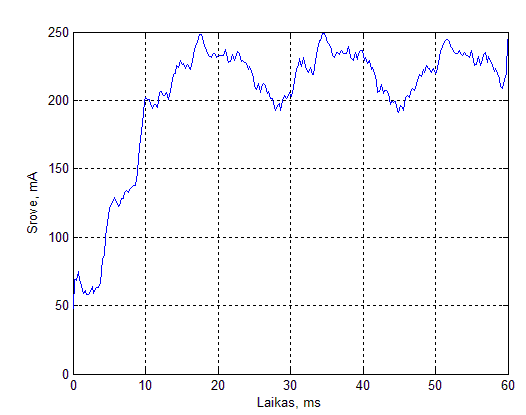
\includegraphics[width=400px]{img/head_tracker_5min.png}
  \caption{Galvos orientacijos sekimo įrenginio vartojamos elektros srovės priklausomybė nuo laiko po 5 minučių darbo.}
  \label{fig:headtracker_5min}
\end{figure}

Kaip matoma iš \ref{fig:headtracker_5min} paveikslo, elektros srovės suvartojimas įrenginio įjungimo metu, bet po 5 minučių darbo padidėja. Taip yra todėl, kad galvos orientacijos sekimo įrenginio temperatūra po 5 minučių darbo šiek tiek pakyla. Srovės suvartojimo padidėjimas siekia maždaug 20 mA.

\subsection{Garso apdorojimo įrenginio patikra}

Šis poskiris skirtas apibendrinti garso apdorojimo įrenginio veikimą bei jo charakteristikas.

\subsubsection{Energijos suvartojimo patikra}

\ref{fig:sound_energy} paveiksle pavaizduota garso apdorojimo įrenginio srovės suvartojimo priklausomybė nuo laiko šalto paleidimo metu.

\begin{figure}[htbp]
  \centering
  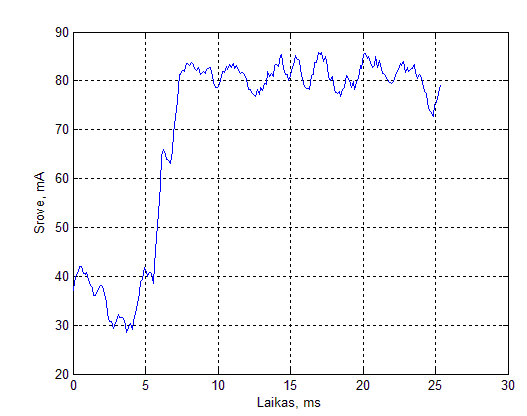
\includegraphics[width=400px]{img/sound_energy.png}
  \caption{Garso apdorojimo įrenginio vartojamos elektros srovės priklausomybė nuo laiko šalto paleidimo metu.}
  \label{fig:sound_energy}
\end{figure}

Kaip matome iš \ref{fig:sound_energy} paveikslo maksimalus elektros srovės suvartojimas siekia iki 85 mA. Didžiąją dalį šios srovės suvartojimo sudaro įtampos stabilizatorius. Likusias dalis – mikrovaldiklis ir skaitmeninis-analoginis keitiklis. \ref{fig:sound_energy_5min} paveiksle pavaizduota srovės suvartojimo priklausomybė nuo laiko įjungimo metu po 5 minučių įrenginio darbo.

\begin{figure}[htbp]
  \centering
  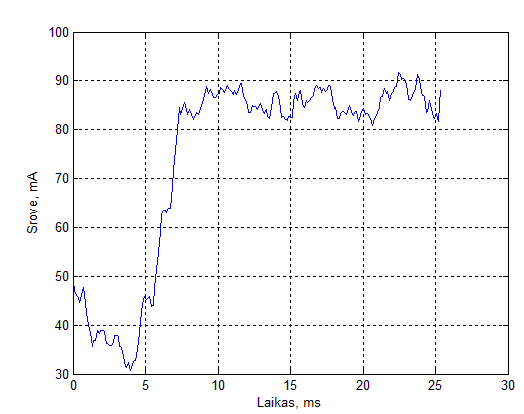
\includegraphics[width=400px]{img/sound_energy_5min.png}
  \caption{Garso apdorojimo įrenginio vartojamos elektros srovės priklausomybė nuo laiko po 5 minučių darbo.}
  \label{fig:sound_energy_5min}
\end{figure}

Kaip matome iš \ref{fig:sound_energy_5min} paveikslo, garso apdorojimo įrenginio srovės suvartojimas po 5 minučių įrenginio darbo padidėja tik apie 5 mA. Taip yra todėl, kad įtaisas yra geriau suprojektuotas ir neatsiranda nereikalingų įtampos kritimų, o tuo pačiu ir energijos išsklaidymo šilumos pavidalu. Taip pat čia nėra duomenų perdavimo modulio \textit{BTM222}, kuris suvartoja gana nemažai elektros energijos.

\newpage

\subsection{Išvados}
Išvada – garso apdorojimo įrenginys mažiau kaista, lyginant su galvos orientacijos sekimo įrenginiu bei mikrovaldiklis ir periferija maitinami 3.3 V elektros įtampa, todėl įtaisas yra ganėtinai ekonomiškesnis.
Kol kas visos sistemos elektroninė dalis yra tik prototipo stadijoje, todėl visi atlikti matavimai yra preliminarūs ir ateityje keisis. Visos sistemos maksimalus elektros srovės suvartojimas tesiekia tik apie 340 mA, o tai atitinka užduoties rėžius (500 mA). Esamą srovės suvartojimą dar galima sumažinti minėtais būdais skyriuje, bet tai yra ateities planai ir šiuo metu tai nėra ypatingai aktualu, norint įrodyti ir pademonstruoti sistemos veikimą.

\end{document}